\tightsection{Quality Improvement via Prediction}
\label{improvement}
%Now we can fill in the details of section 3 a bit more.  Figure~\ref{fig:go-overview} shows how prediction and decision-making work in GO.
Having shown that with the attributes we collect, our prediction algorithms can provide close-to-optimal prediction accuracy, we now examine the quality improvement resulting from the prediction algorithms. Providing that our prediction algorithm is roughly accurate, GO's ``transition'' from prediction accuracy to quality improvement is straightforward -- it simply chooses the decision that has the best predicted quality. 

Since improving video quality is the ultimate goal of GO, we would like to quantify the impact of prediction algorithms on quality improvement. Specifically, we would like to answer two questions:
\begin{packedenumerate}
	\item How much quality improvement does GO make under various scenarios?
	\item How does prediction accuracy impact quality improvement under realistic scenarios?
\end{packedenumerate}

The difference between two questions is that the first question quantifies the impact of different scenarios on quality improvement with a fixed solution, i.e., GO. The second question quantifies the impact of the goodness of solution (i.e., prediction accuracy) on quality improvement, in realistic scenarios. This section begins with our methodology to answer the two questions. Then, we present our results and observations of each question.

\tightsubsection{Methodology}
To answer these two questions, we need to have three types of input. Here we briefly describe their intuition and difference. We will present the parameters and setup in detail when using them to answer particular questions.
\begin{packeditemize}
	\item {\it Controlled synthetic input:} We need fully controlleable input in which the true outcomes (i.e., ``ground truth'') of multiple decisions are under our control and we can change them continously so as to quantify the quality improvement. By doing so, we would also be able to have access to the optimal quality (i.e., an {\it oracle} approach) which it will be useful to compare GO with.
	\item {\it Counterfactual input:} To answer these questions under realistic scenarios (real trace), we use a methodology similar to A/B testing, which we call {\it counterfactual testing}. The methodology is described in detail in section~\ref{sec:counterfactualtesting}. Its basic idea is that we first collect a dataset (called {\it random dataset}) in which the decisions are randomly made for each client and we collect the quality each client gets. To evaluate the outcome of the same set of sessions with each making a decision based on some algorithm (i.e., possibly the same decision), we will be able to have unbiased evaluation on those sessions with the same decision as in the dataset.
	\item {\it Randomized trace-driven input:} Randomizing real traces with controlled amount is important for evaluating a decision-making algorithm. However, real traces do not admit the sensitivity analysis of a decision-making algorithm to the changes in scenario parameters -- after the input scenarios is changed, the outcome of each session under an alternative decision is unavailable \jc{why counterfactual input won't work}.  To remedy these limitations, we generate a trace-driven synthetic dataset. The basic idea is to generate a session $s$ whose outcome of each decision $d$ is drawn from the distribution of outcomes of this decision $d$ on other sessions exactly matching the same attributes with $s$. Having ensured that quality outcomes in the synthetic scenario are known for any decision, it is possible to identify an {\it oracle} approach that always makes the best decision.
\end{packeditemize}
In any scenario, we would like to quantify the quality improvement of GO based on random selection (which makes decision with equal prabability), and how close GO is to an oracle approach (with controlled and trace-driven synthetic input).

\comment{
\begin{figure}[h!]
\centering
 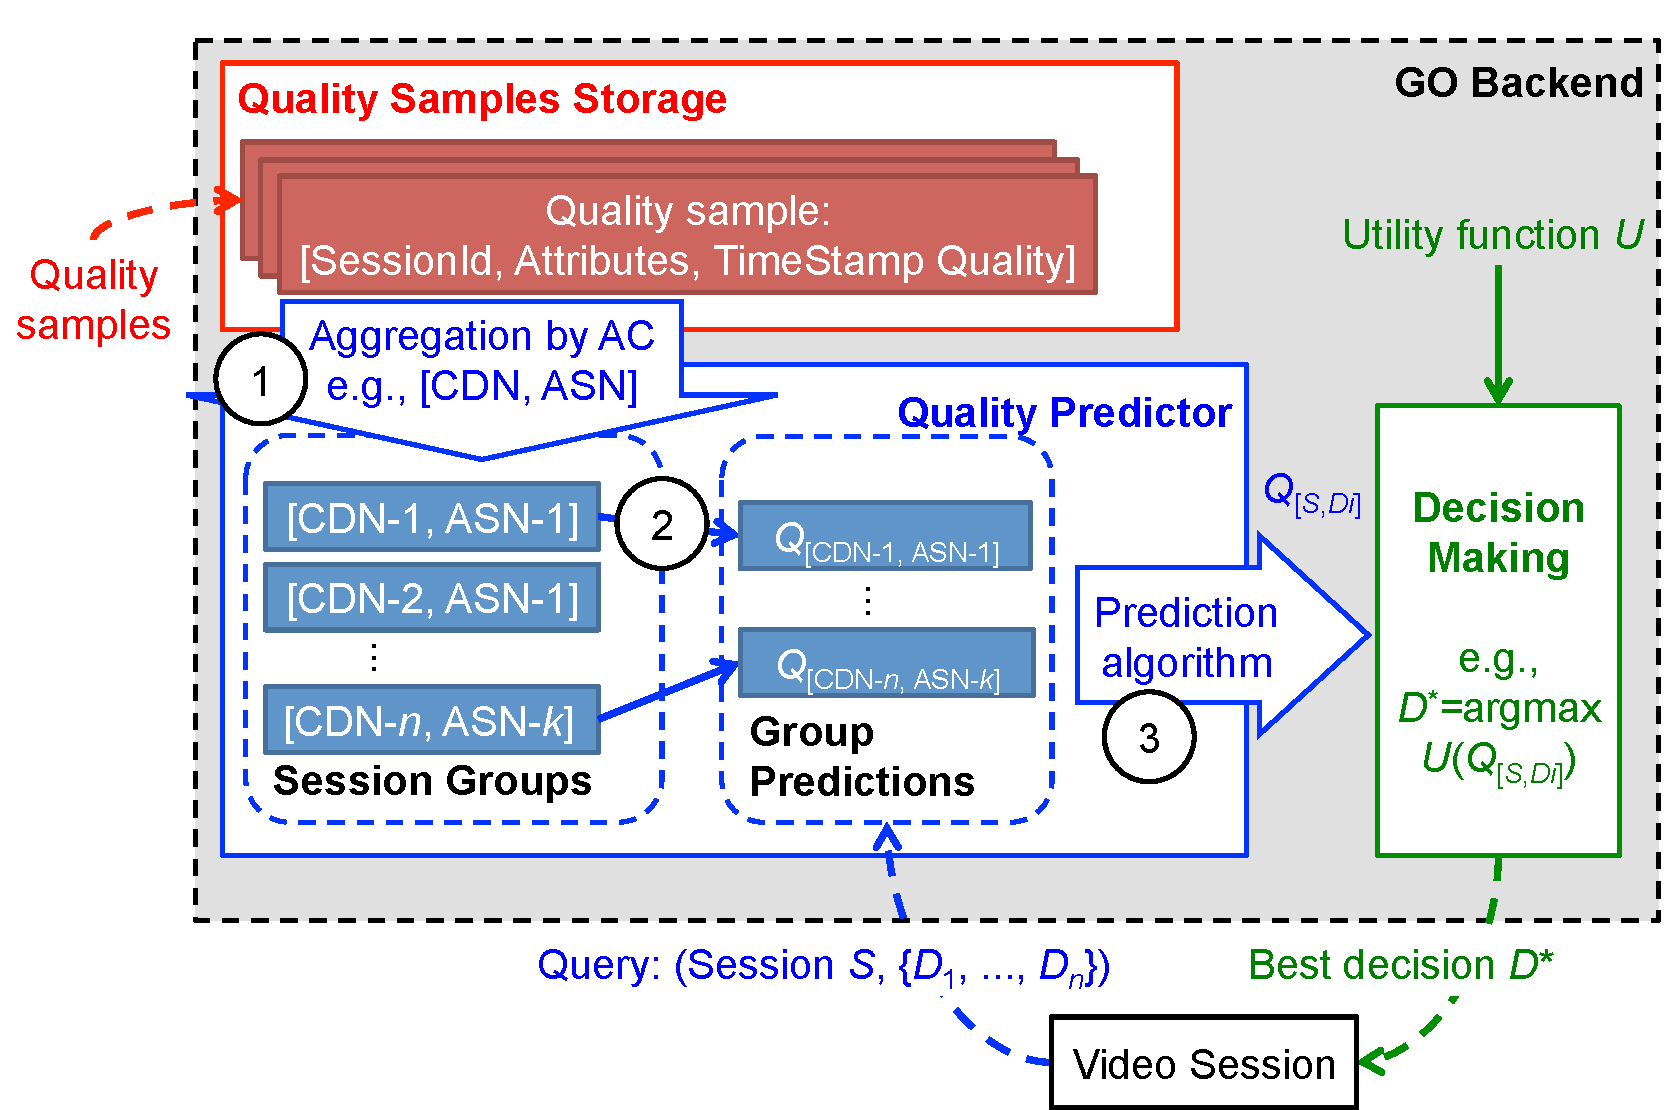
\includegraphics[width=0.3\textwidth] {figures/backend.pdf}
\tightcaption{Schematic overview of GO backend.}
\label{fig:backend}
\end{figure}
}

\tightsubsection{Improving quality with GO}

\tightsubsubsection{Behavioral study}
To build confidence in this algorithm, we use controlled synthetic input to show how decision-making based on prediction behaves in some simple synthetic scenarios where the optimal decisions are clear:
\begin{packedenumerate}
  \item {\it CDN performance degradation.} A sudden change in CDN performance causes relative performance to change.
  \item {\it Client-side vs. server-side bottleneck.} 
\end{packedenumerate}

\begin{figure}[h!]
\centering
 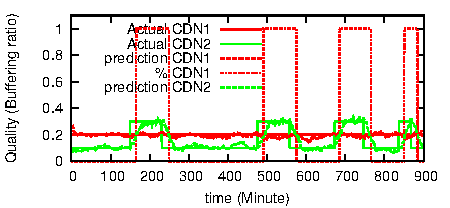
\includegraphics[width=0.5\textwidth] {figures/behavior-evaluation/simple-change.pdf}
\tightcaption{Behavioral study: CDN performance degradation.}
\label{fig:cdn-degradation}
\end{figure}

\tightsubsubsection{Evaluation under real trace}
We show how GO works in practice in a real trace, in comparison to a naive baseline algorithm that makes random decisions.  Here we use a methodology similar to A/B testing, which we call {\it counterfactual testing}; the methodology is described in detail in section \ref{sec:counterfactualtesting}.  The dataset is described in section \ref{subsec:dataset}.  Results are displayed in figure \fillme; we can see that \fillme.

\begin{figure*}[t!]
\centering
\subfigure[Buffering ratio]
{
        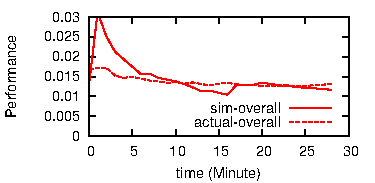
\includegraphics[width=0.23\textwidth]{figures/counterfactual/result-a-overall-metric0.pdf}
}
\subfigure[Average bitrate]
{
        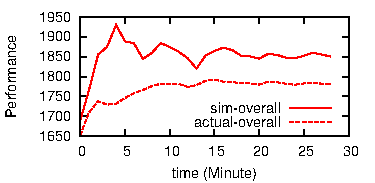
\includegraphics[width=0.23\textwidth]{figures/counterfactual/result-a-overall-metric1.pdf}
}
\subfigure[Join time]
{
        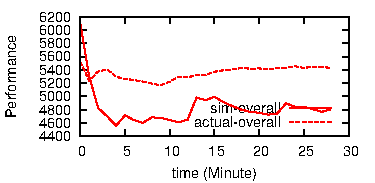
\includegraphics[width=0.23\textwidth]{figures/counterfactual/result-a-overall-metric2.pdf}
}
\subfigure[Start failure rate]
{
        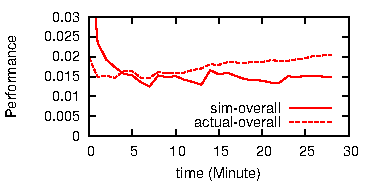
\includegraphics[width=0.23\textwidth]{figures/counterfactual/result-a-overall-metric3.pdf}
}
\tightcaption{Counterfactual input. Evaluation under real trace}
\label{fig:counterfactual}
\end{figure*}

\tightsubsubsection{Impact of quality heterogeneity}
To control the quality heterogeneity, we randomize the real trace to create a randomized trace-driven input. \fillme \jc{it's still not clear to me how we change the quality outcome}



%Randomized experimentation in real traces is the most important way to evaluate a decision-making algorithm.  However, real traces have a few limitations.  In real traces, it is impractical to identify an optimal alternative against which to compare GO, so that we can understand how close it is to the best algorithm.  In addition, real traces do not admit simple analysis of the sensitivity of a decision-making algorithm to the changes in scenario parameters.  To remedy these limitations, we generate a synthetic dataset from our real data.  We do this using a simplifying assumption: We fix a set of attributes $g$, and assume that conditional on a session belonging to a group under this AC, its quality outcomes given each decision are statistically independent.  Essentially this amounts to an assumption that we observe all interesting attributes.  \fillme.

%Under this assumption, we can generate a new session from the same distribution that generated a real dataset as follows: Sample uniformly at random from the sessions we observed.  The synthetic session has the same attributes, denoted $a_i$, as the sampled session.  We assign quality outcomes to each possible decision by sampling uniformly at random from the quality outcomes observed for sessions with attributes exactly matching $a_i$.  Crucially, this ensures that quality outcomes in the synthetic scenario are known for any decision, not just the decision that was actually taken for a session.  In particular, it is possible to identify an {\it oracle} for this scenario that makes perfect predictions of quality outcomes for any decision.

% [The following is an unfinished writeup for old synthetic scenario scheme:]
%The scenario is generated as follows: The scenario lasts for $T$ minutes.  Each session is assigned values on four different attributes, $A_0, A_1, B_0,$ and $B_1$, and lasts for $1$ minute.  Each unique attribute combination (i.e. each group) $a$ is associated with some static parameters and some parameters that change over time, which inform the generation of sessions in that group:
%\begin{packedenumerate}
%  \item $n_{a}$: The number of sessions in this group.
%  \item $\mu_{atj}$: The average quality outcome for sessions in this group, when decision $j$ is taken.
%  \item $\sigma_{atj}$: The standard deviation of quality outcomes for sessions in this group, when decision $j$ is taken.
%\end{packedenumerate}
%
%For each minute $t$, sessions are generated as follows: Group $a$ has $n_{a}$ sessions.  The $i$th session in group $a$ has attribute values $a$.  There are $J$ possible decisions; each session has quality outcome $q_{itaj}$ drawn from the distribution $\operatorname{Normal}(\mu_{atj}, \sigma_{atj}^2)$, for each decision $j$.  The actual decision $d_{ita}$ for the session, which is used to populate the quality sample used in GO, is chosen uniformly at random from among the $J$ possible decisions.

%\tightsubsubsection{Evaluation against an oracle using synthetic data}
%Here we compare GO against the oracle (and against a random decision-maker) in our synthetic scenario.  \fillme.
%
%We also check the sensitivity of GO to the true difference in quality between decisions.  We do this by shifting the distribution of true quality outcomes in varying degrees.  \fillme.

\tightsubsection{Understanding the impact of prediction accuracy on quality improvement}

Separately from the GO algorithm, it is also interesting to see how prediction error generically impacts quality outcomes.  To control the prediction accuracy in real trace, we have to identify the true outcome of decisions we did not take. Therefore, we use randomized trace-driven input. The key challenge is given a session $s$ and one of its decisions $d$, to draw the outcome from the distribution $M_{v_g(s),d}$ of outcomes of this decision on other sessions that share the same attributes with this session. Remember $v_g(s)$ returns the values on all attributes in $g$ of session $s$. We investigate two ways of doing so. 
\begin{packedenumerate}
	\item Unproprtional: The outcome is uniformly at random from $M_{v_g(s),d}$. Its underlying assumption is that we observe all attributes that determine the quality, so that with the same decision, the quality of sessions that match all attribute is random values with unbias noise.
	\item Proportional: For a session $s$, if the outcome of $d_1$ is in the $q$-quantile of $M_{v_g(s),d_1}$, the outcome of $d_2$ is also in the $q$-quantile of $M_{v_g(s),d_2}$. Its underlying assumption is that there is unobserved attributes that determine the quality, so that if the session performs poorly in one decision, it will also be bad on other decisions.
\end{packedenumerate}

We control the prediction accuracy by generating prediction such that the prediction deviates from the real outcome by an independent random Gaussian noise of varying magnitude. 

\begin{figure}[h!]
\centering
 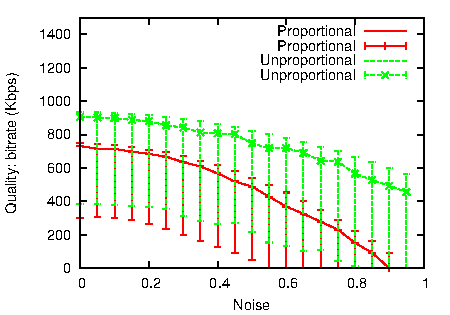
\includegraphics[width=0.3\textwidth] {figures/impact/result-noise-impact.pdf}
\tightcaption{Impact of noise on quality. GO prediction gives 3300Kbps (unproportional) and }
\label{fig:cdn-degradation}
\end{figure}

%Here it is important to identify an oracle predictor as a baseline, so we use the same synthetic scenario as above.  We add random independent Gaussian noise to the oracle's predictions (an admittedly crude model of prediction error) and show how larger amounts of noise impact quality outcomes.  Figure \fillme displays this.  We can see that quality improvement is unaffected by small amounts of prediction inaccuracy but drops off quickly at a (scenario-dependent) threshold \fillme.

%We cannot subtract noise from GO's predictions in a real scenario, since we do not know the true outcome of decisions we did not take.  However, we can {\it add} noise to GO's predictions and observe the impact of {\it worse} prediction on quality outcomes.  As above, we use independent random Gaussian noise of varying magnitude.  Figure \fillme displays this for our synthetic scenario, and figure \fillme displays it for a real trace.  In the synthetic scenario, GO's performance in quality improvement is equivalent to that of an oracle with \fillme random noise.  \henry{We hope to see that decreasing prediction accuracy eventually leads to highly degraded performance.}